\documentclass[11pt,oneside,a5paper]{report}
\usepackage{natbib}
\usepackage{breakcites}
\usepackage{microtype}
\usepackage[vcentering,dvips]{geometry}
\geometry{papersize={7in,9in},bottom=3pc,top=5pc,left=5pc,right=5pc,bmargin=4.5pc,footskip=18pt,headsep=25pt}
\pdfobjcompresslevel=0

\usepackage[tocindentauto]{tocstyle}
\usetocstyle{standard}
\setcounter{tocdepth}{1}
\usepackage[nottoc]{tocbibind}
\setcounter{secnumdepth}{3}

\pagestyle{headings}
\setlength{\parskip}{0.25 \baselineskip}

\usepackage{amsmath}
\usepackage{amssymb}
\usepackage{bm}
\usepackage{subcaption}
\usepackage{graphicx}
\usepackage{svg}

\title{\textbf{Hilbert Spaces as Generalized Conceptual Spaces} \\
in Information Dynamics of Thinking Theory}
\author{Steve Homer}
\date{}

\def\innerproduct{\langle\cdot _, \cdot\rangle}
\def\orthseq{\{ \varphi_n \}_{n=0}^\infty}

\begin{document}
\maketitle
\tableofcontents

\chapter{Introduction}
\include{tex/introduction/introduction}
\include{tex/introduction/context}
\include{tex/introduction/problem-justification}
\include{tex/introduction/objectives-hypotheses}
\include{tex/introduction/research-method}
\section{Structure}
\label{section:structure}

Following this introduction, the structure of the thesis is as follows:

\textbf{Chapter 2: Background:} First, a few short sections of background information regarding conceptual spaces, Hilbert spaces, and information theory will be explained. These are necessary to understand the final background section, Information Dynamics of Thinking, of which this thesis is an implementation.  This section will give the motivations for IDyOT theory as a cognitive architecture and explain its main principles of information dynamics and efficiency.  It  will also outline the main processes of segmentation, categorization, and abstraction core to the functioning of IDyOT.

\textbf{Chapter 3: Theory \& Implementation:} Following the high-level description of IDyOT, more specific matters of theory stemming from the chosen formalisms will be covered.  Explications of utilizing Hilbert spaces and the Fourier transform are explored in the Abstraction and Segmentation sections, whereas the Categorization and Interpolation sections round out the chapter in implementation, tying everything together.

\textbf{Chapter 4: Empirical Analysis:}  The implemented system described in Theory \& Implementation is then empirically tested on a corpus of human speech, with the results visualized to allow for qualitative evaluation against human speech.  These visualizations are explained in the context of IDyOT with the preliminary results suggesting that the different processes of IDyOT are behaving as envisioned in the theory.

\textbf{Chapter 5: Evaluation \& Discussion:} After looking at the specifics of the results in the Empirical Analysis, the overall strengths and deficiencies of both the theory and implementation are investigated in the Discussion, finding that though certain aspects of the results of the implementaion are inconsistent, overall, the implementation at least partially confirms the theory.  After this, the broader implications of IDyOT as a general approach to perceptual representation will be examined.

\textbf{Chapter 6: Conclusion:} Finally, the contributions and limitations of not only the implementation but also the theory are summarized, finishing with prospects for future work that can expand the semantic range of the implementation through the use of different geometries and transformations.


\chapter{Review}
\include{tex/review/review}
\chapter{Comparisons}

\section{Mel-Frequency Ceptral Coefficients (MFCCs)}

\section{Transformer Architecture (in NLP)}


\chapter{Background}
\include{tex/background/background}
\section{Conceptual Spaces}
\label{section:conceptual-spaces}

In knowledge representation, the argument over the representation of cognition often falls into two camps: connectionism and symbolicism.  As the lowest level of represention, connectionism is best exemplified by artificial neural networks, where cognition emerges from myrid connections between neurons.  At the highest level, symbolicism views the mind as a Turing machine \cite{turing2009computing}, where cognition is equivalent to compution by symbol manipulation.  Conceptual spaces theory \cite{gardenfors2004conceptual} argues for a middle way, through the use of so-called conceptual spaces.  Conceptual spaces theory views cognition as the process of concept formation by means of similarity, so that the continuous representations of connectionism can be bridged to the discrete representations of symbolicism, hopefully gaining the best of both worlds.  

Conceptual spaces theory places objects into so-called conceptual spaces -- semantically rich spaces with geometric properties -- which allow for intuitive geometric reasoning about related objects. For instance, in the conceptual space of color with dimensions of hue, saturation, and brightness, one can formally make a geometric claim that “orange lies between yellow and red.”  This simple claim cannot be made by connectionism or symbolicism without imposing ad-hoc external semantics on the neural connections or symbols respectively, highlighting the explanatory power of conceptual spaces for knowledge representation.

\subsection{Quality Dimensions}
\label{subsection:quality-dimensions}

Quality dimensions are the basic building blocks of a conceptual space.  They can be thought of as the axes that give meaning to the elements in the space.  In three-dimensional Cartesian space, when referring to a point, we specify it by its placement on each of the $x$, $y$, and $z$ -axes.  By analogy, each of the $xyz$-axes would be a quality dimension in the 3D Cartesian space.  However, quality dimensions are more than just orthogonal unit vectors, they can also have their own specific geometry that serves to constrain the dimension. For instance, a quality dimension may have the geometry of a circle, resulting in different behavior than the real number line.  Quality dimensions also allow us to speak meaningfully about similarity between objects in a space since, by definition, they possess distance and betweenness relations.  Finally, it is important to remember that the 'quality' of the quality dimension is what gives it inherent semantic content beyond just being a descriptive dimension.

\subsection{Domains and Conceptual Spaces}
\label{subsection:domains-and-conceptual-spaces}

Integral quality dimensions require one another to exist.  For instance, the three qualities of sound: pitch, timbre, and loudness, are all integral to one another.  It is impossible to identify a sound without specifying all three of these dimensions.  On the other hand, most quality dimensions are separable, meaning that they are independent of one another.  Though separable quality dimensions are independent, they may still be highly correlated, which may give the illusion that they are integral.

A domain is a set of integral dimensions that are separable from all other dimensions.  In a sense, it is the minimum description needed for a given space.  For example, the three qualities of sound form a domain.  Often, different domains will be correlated with one another, and combining them will yield a richer description of a given object.  This combination of multiple domains is what is referred to as a conceptual space, so that the specification of an object is nothing else but its location in a conceptual space.

\subsection{Similarity, Distance, Betweenness}
\label{subsection:similarity-distance-betweenness}

Humans have an innate sense of similarity without being able to fully describe why two things are similar (cite?).  In simple cases, this similarity can be made explicit, for example that a rectangle is more similar to a square than a circle.  However, this intuition for similarity extends to even very abstract realms.  For instance, most people would naturally agree that country music is closer to rock-n-roll than it is to classical Indian ragas, but would be hard-pressed to give an exact definition or method of why this is so.

Conceptual spaces allow this innate sense of similarity to be codified in the intuition of geometry, betweenness, and distance.  Given a betweenness relation for a conceptual space, one can say that a given object is between two other objects, which allows us to say that one is closer to another than the third.  In our case, we will study conceptual spaces equipped with a distance measure.  This allows us to examine similarity between objects, such that more similar onjects will be closer to one another than more different objects.

\subsection{Convexity of Properties and Concepts}
\label{subsection:convexity-properties-concepts}

Given that Conceptual Spaces Theory posits that cognition is equivalent to the formation of concepts \cite{gardenfors2004conceptual}, one should define a concept.  Defining a property or context as "an invariance across a range of contexts, [reifiable] so that it can be combined with other appropriate invariances" \cite{kirsh1991today}, it is immediately clear that these correspond to regions of a conceptual space.  Since all of the objects in a given region are similar to each other, by grouping them together as a region, we can see that the region corresponds to a property or concept.  A property would be a region in a domain -- for instance the red property corresponds to a region of the color space -- and a concept would be a region in a conceptual space.

Gardenfors \cite{gardenfors2004conceptual} posits that regions corresponding to properties and concepts are convex in nature.  Though this does not fall directly from the theory itself, it is reasonable to think that the region of concept is not intruded upon by other concepts.  For example, in the color space, the property of red is convex, since we don't see another color like blue interloping into the red region, which would appear as a small area of blue surrounded by a region of red.

\subsection{Higher-order Conceptual Spaces}
\label{subsection:higher-order-conceptual-spaces}

Higher-order conceptual spaces can be created from combinations and transformations of one or more lower-order conceptual spaces \cite{gardenfors2004conceptual}.  The key notion of the higher-order nature of these spaces is that they are more abstract than the spaces they are generated from.  This is to distinguish higher-order conceptual spaces from combinations that serve to more tightly constrain a space, similar to an intersection set operation.  For instance, overlaying the full color space over the space of human phenotypes results in a restricted color space of human skin tones, not a more abstract space.

Since by nature, quality dimensions and domains often describe low-level quantities like color and sound, it is necessary to combine them into more abstract spaces that yield higher-level spaces with more explanatory power.  Intuitively, the higher level a given conceptual space is, the richer its semantics, so to arrive at a space with sufficient descriptive capabilities for a given cognitive representation, it may be necessary to recursively abstract conceptual spaces into higher-order spaces to arrive at something nontrivial with interesting semantics.

\section{Hilbert Spaces}
\label{section:hilbert-spaces}

\begin{quote}
  "Hilbert spaces are the means by which the ordinary experience of Euclidian concepts can be extended meaningfully into the idealized constructions of more complex math." \cite{bernkopf2008schmidt}
\end{quote}

Originally, conceptual spaces \cite{gardenfors2004conceptual} were formalized by using Euclidian or Manhattan distances to measure similarity in conceptual spaces modeled in constrained Cartesian space. Though this is useful in building an intuition as to how conceptual spaces operate in practice, it can be limiting in the description of relations between objects and the space itself.  In order to allow for more flexibility in this regard, we need a more general notion of a space than a finite-dimensional Euclidian space.  The generalization employed here is that of Hilbert spaces, most famously applied as the foundation of quantum mechanics \cite{neumann1955mathematical}, but with numerous applications in a variety of fields \cite{kennedy2013hilbert}.

\subsection{Complete Inner Product Space} 
\label{subsection:complete-inner-product-space}

A Hilbert space is defined as a complete inner product space.  That is, a Hilbert space is a vector space equipped with an inner product $\innerproduct$, but is also complete: the space is big enough to include the norm of converging sequences.  In the case of an infinite-dimensional Hilbert space, this completeness criterion cannot be taken for granted, but in the finite-dimensional case, the space is always complete.  The inner product of a Hilbert space induces a norm $\|f\| = \langle f, f \rangle^{1/2}$, which allows us to talk about distances between vectors, something that we require in a generalized formalism of conceptual spaces.

What makes Hilbert spaces powerful is the ability to represent a function as a point in the space.  With the aid of the inner product, one can produce an (infinite) orthonormal sequence $\orthseq$ for the Hilbert space.  By decomposing any function $f$ into its Fourier series (equation \ref{equation:fourier-series}) on that sequence, we can recover a corresponding coefficient $\langle f, \varphi_n \rangle$ for each element of the orthonormal sequence.

\begin{equation} 
  \label{equation:fourier-series}
  f = \sum_{n=0}^\infty \langle f, \varphi_n \rangle \varphi_n
\end{equation}

By arranging each of these coefficients into a vector with dimensions $\varphi_n$, the function can be represented as a point in the Hilbert space. If that space is finite, we can equivalently represent a point $x$ in the Hilbert space as an array of complex numbers, $x \in \mathbb{C}^n$ where $n$ is the number of dimensions.

\subsection{Application to Conceptual Spaces}
\label{subsection:application-conceptual-spaces}

Now, by defining a conceptual space formally in terms of a Hilbert space, we see that the geometry of the conceptual space can be fully defined by the inner product of the Hilbert space.  This has two consequences.  First, since for a given function, the Fourier series decomposition generates a vector representation, any number of different vectors can be produced from the same function for each inner product.  This means that a given object can be represented in any number of conceptual spaces defined by their inner product.

Conversely, since it can be proven that all Hilbert spaces of the same number of dimensions are isomorphic \cite{kennedy2013hilbert}, given a vector, we can then choose an inner product to determine its representation.  In this way, each inner product imposes a geometry that allows for different perspectives of the same "raw" data.  By analogy, in figure \ref{figure:cartesian-radial} we see that coordinates represented on $(x, y)$ in a 2D Cartesian space have a different meaning and location than if they are represented on $(r, \theta)$ in a 2D radial space.  This allows for complete flexibility in representation, as an object can be placed in a conceptual space simply by interpreting its vector representation according to the inner product of that space. \cite{wiggins2018creativity}

\begin{figure}
  \centering
  \begin{subfigure}[H]{0.45\linewidth}
    \def\svgwidth{\linewidth}
    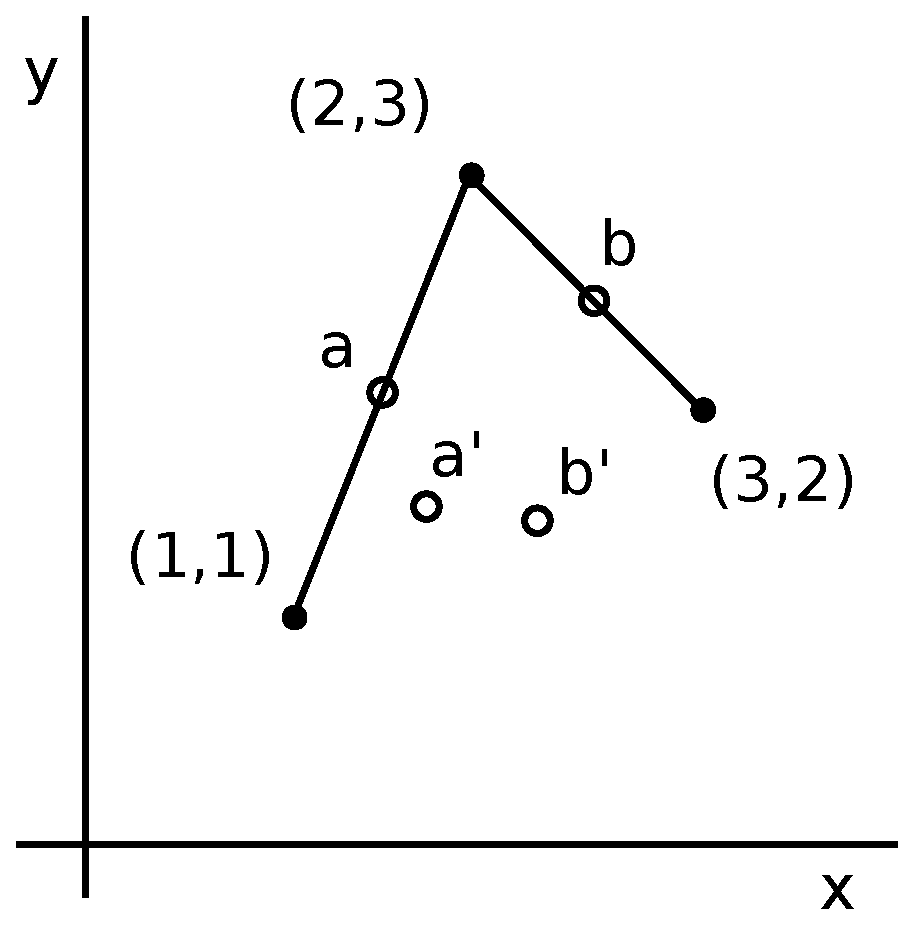
\includegraphics[width=\linewidth]{fig/interpolation-cartesian.eps}
    \caption{2D Cartesian Space}
  \end{subfigure}
  \begin{subfigure}[H]{0.45\linewidth}
    \def\svgwidth{\linewidth}
    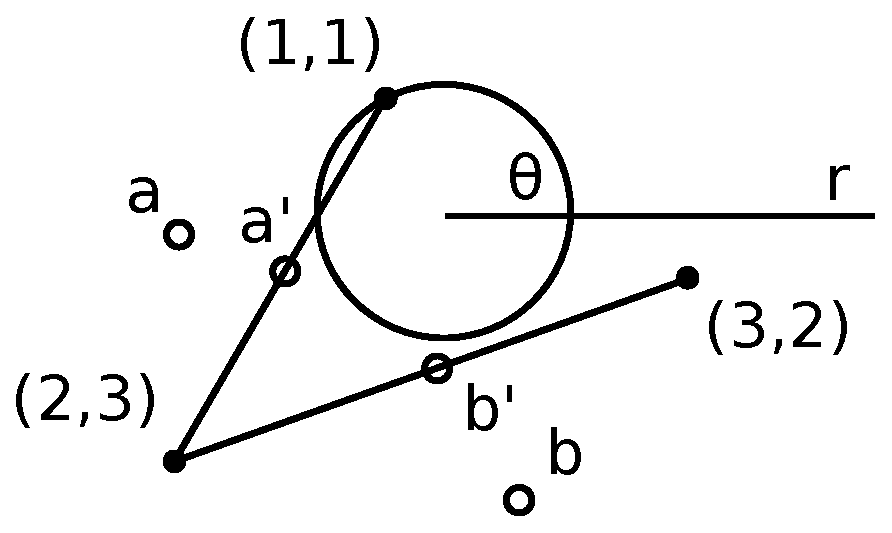
\includegraphics[width=\linewidth]{fig/interpolation-radial.eps}
    \caption{2D Radial Space}
  \end{subfigure}
  \caption{Example of effect of spatial geometry on location of coordinates}
  \label{figure:cartesian-radial}
\end{figure}

\section{Information Theory}
\label{section:information-theory}

Shannon's information theory \citep{shannon1948mathematical}, though originally aimed at providing a theoretical foundation to signal processing and communication, has become foundational in all aspects regarding information.  According to information theory, the amount of information in a signal can be thought of as the amount of surprise at seeing a given quantity in that signal.  Put more simply, suppose you come in late to work one morning, and upon arriving into the office, your boss tells you about the weather. No information was gleaned from the conversation, since you already knew the weather from being outside.  If instead, upon entering the office late, your boss fires you on the spot, you would be very surprised, learning something unexpected, and gaining a lot of information.

\subsection{Entropy}
\label{subsection:entropy}

Entropy $H$ is the measure of information in a probability distribution.  If applied to a discrete signal of symbols, it can be used to represent the amount of information of the signal (equation \ref{equation:entropy}), by taking it over the frequencies of each symbol $s$ of the alphabet $A$.  Entropy is then the number of bits required to represent each symbol without ambiguity.

\begin{equation}
  \label{equation:entropy}
  H(A) = - \sum_{s \in A} p(s) \log_2 p(s)
\end{equation}

\subsection{Information Content}
\label{subsection:information-content}

Though entropy is useful in describing the quantity of information of an entire distribution, to find the information content $h(s)$ of a single symbol in an alphabet, one must use equation \ref{equation:information-content} below \citep{mackay2003information}. Since some symbols are less likely to occur than others, observing them gives more information than more likely ones, which is reflected here.

\begin{equation}
  \label{equation:information-content}
  h(s) = - \log_2 p(s)
\end{equation}

Whereas information content looks at a symbol in isolation, conditional entropy looks at symbols in pairs.  Conditional entropy is equivalent to the information content of a symbol, given that another symbol is known.  If we are referring to a stream of symbols, the conditional entropy would be the information content of a symbol given that we just saw the previous symbol.

\begin{equation}
  \label{equation:conditional-entropy}
  H(s|t) = -\log_2 p(s|t)
\end{equation}



\chapter{Inductive Constraints}
Multiple levels of abstraction constrain one another

Major references:
The acquisition of Inductive Constraints (Kemp),
The Discovery of Structural Form (Kemp, Tenenbaum),
Hierarchical Bayesian Models and Hierarchical Markov Models

\section{Information Dynamics of Thinking}
\label{section:idyot}

Cognitive architecture blending information theory and conceptual spaces.

\subsection{Boundary Entropy Segmentation}
\label{subsection:boundary-entropy-segmentation}

In natural language processing, n-gram models are often employed to track the frequency of chains of symbols in a given signal.  For instance, if examining textual data, a unigram model would count the frequency of individual words, whereas a bigram model would track the frequency of pairs of words.  It is clear that one can then utilize the information content measure on a unigram model and the conditional entropy measure on the bigram model in order to quantify the amount of information in that model. \cite{sproat1996stochastic}

\subsection{Sequential Memory}
\label{subsection:sequential-memory}

The sequential memory in IDyOT is represented as a hierarchy of chains of symbols. As the agent perceives a continuous stream of perception from the environment, it first discretizes that stream into moments, and links those discretized percepts as symbols in an ever-growing chain.  By examining time-varying information-theoretic properties of this chain, it can be chunked into a series of segments composed of a sequence of symbols.  This segment can then be abstracted by a representative symbol in the superior layer and can be said to subsume the inferior segment.  This process is done recursively until no more abstraction can be performed.

\subsection{Spectral Representations of Meaning}
\label{subsection:semantic-spectral-representation}

\subsection{Semantic Memory}
\label{subsection:semantic-memory}

If the sequential memory can be though of as how concepts relate to eachother over time, semantic memory can be thought of as how those concepts relate to eachother outside of time.  In IDyOT this is modeled using conceptual spaces.  At any given layer of abstraction in the sequential memory, there is a "parallel" semantic space for the symbols of that layer.  This allow us to think of a segment of symbols in sequential memory as a trajectory of concepts in semantic memory.  By looking at a spectral representation of this trajectory, the time-varying properties of the segment are removed, and this spectral representation can be thought of as an abstraction of the segment, and therefore as the abstracted symbol in the superior layer of the sequential memory.


\chapter{Theory}
\include{tex/theory/theory}
\section{Abstraction}
\label{section:abstraction}

When a segment is produced in the segmentation process, it is abstracted to a single symbol in the superordinate abstraction layer.  Since each dimension is composed of both an alphabet of symbols and a conceptual space in which those symbols live, a memory sequence is at once a segment of symbols in the sequential memory as well as a trajectory through the corresponding conceptual space in the semantic memory \citep{wiggins2019learning}. Since here we will utilize the formalism of finite-dimensional Hilbert spaces to model conceptual spaces, this trajectory corresponds to a time-parametric curve in a high-dimensional space.

\subsection{Fourier Transform}
\label{section:fourier-transform}

In the abstraction process, we would like to produce a spectral representation of a segment.  Here, we will apply the discrete Fourier transform (DFT) operator \citep{cooley1965algorithm} to the discrete trajectory (see equation \ref{equation:discrete-fourier-transform}), taking it from the time-domain $n$ to the frequency-domain $k$.  Though there are other spectral operators, there is evidence, especially in the auditory domain, that the brain operates on frequency transformations of time-varying signals from the Organ of Corti \citep{moore2012introduction}, and so it is employed here.  

\begin{equation}
  \label{equation:discrete-fourier-transform}
  \mathcal{F}_D [x_n] = X_k = \sum_{n=0}^{N-1} x_n e^{-\frac{i 2 \pi}{N} kn}
\end{equation}

By taking the Fourier transform (equation \ref{equation:fourier-transform}) of a time-varying signal $f(t)$, we produce the frequency-domain signal $F(\xi)$ for each orthogonal frequency.  So by taking the Fourier transform of a curve in a Hilbert space, we end up with a spectral representation of that curve.  The abstraction process will then consist of taking the Fourier transform of a trajectory through a Hilbert space, and then viewing the resulting frequency-domain signal as a point in the superordinate space.

\begin{equation}
  \label{equation:fourier-transform}
  \mathcal{F} [f(t)] = F(\xi) = \int_{-\infty}^\infty f(t) e^{-i 2 \pi \xi t} dt
\end{equation}

\subsection{Tensor Rank Promotion}
\label{section:tensor-rank-promotion}

The Fourier transform is an integral operator on Hilbert spaces \citep{kennedy2013hilbert}.  Since operators, by definition, take a function as input and produce a function as output, when thinking in terms of finite-dimensional Hilbert spaces, an operator will take the input from one domain to another, but will not change the shape of that input.  For example, if each point is represented as a vector, a sequence of those points would be a vector of vectors, i.e. a matrix.  Since we view the result of the Fourier transform as a point in the superordinate space, in our example, the point is now represented as a matrix.  Therefore, the result of abstracting a trajectory of points in a subordinate layer is a point in the superordinate space with one higher rank.  Hence, each level of abstraction promotes the rank of its constituent tensors by one. 

To clarify the first few stages of this process, consider Figure \ref{figure:tensor-rank-promotion}. The \textit{Element} row represents the constituent elements of layer $\alpha$.  The \textit{Trajectory} row strings those elements together, and the \textit{Spectral} row shows the shape of the spectral representation of that trajectory after the Fourier transform.  This spectral representation then becomes the constituent element of the superordinate abstraction layer $\alpha+1$.

We begin at the base abstraction layer with a space filled with the raw discrete scalar signal values for each moment of time.  By lining up these values and taking their Fourier transform, the resulting spectral representation is a vector.  This spectral representation is placed into the $\alpha=1$ abstraction layer, whose space is filled with points representing the frequencies of a signal of a short moment of time.  These points are vectors (rank 1 tensors) that, when strung together into a trajectory, form a matrix.  By taking the Fourier transform of this matrix and viewing the result as a point in the superordinate abstraction layer, that upper layer is now composed of points represented as matrices (rank 2 tensors).  Again, we string these points together as a trajectory, but now forming a cube.  By taking the Fourier transform, and viewing it as a point in the superordinate layer, that layer is now composed of points represented as cubes (rank 3 tensors). Repeating this process, we then get hypercubes of increasing rank at each layer of abstraction.  In this manner, the rank of a representative tensor increases by one for each layer of abstraction.

Unfortunately, this leads to an exponential explosion in the number of elements constituting a point in a given layer.  Formally, the number of elements is $r^\alpha$, where $r$ is the resolution of interpolation (see section \ref{section:interpolation}), and $\alpha$ is the level of abstraction.  Though this is not a problem in theory, it has consequences in terms of implementation.

\begin{figure}
  \centering
  \includegraphics[width=\linewidth]{fig/tensor-rank-promotion.pdf}
  \caption{An illustration of tensor rank promotion for the first 4 levels of abstraction, using an interpolation resolution $r = 4$.  }
  \label{figure:tensor-rank-promotion}
\end{figure}

\subsection{Element-wise Independence}
\label{section:elementwise-independence}

When performing the Fourier transform on a tensor of any rank, it should be noted that each component in the tensor is independent from every other component.  Though this is not necessarily true of tensors in general, due to the particular hierarchical construction of these spaces by means of the DFT, each component is decoupled from the rest.  Starting at the bottom, the time-domain sound signal is transformed into a frequency-domain signal of coefficients in independent frequency bins.  It is this independence that allows us to represent the short-term frequency signal as a point with those frequency bins as dimensions.  Performing the DFT on the trajectory of frequency vectors results in independent frequency bins filled with vectors that possess independent entries, meaning all elements are independent one another.

Hierarchically performing the DFT at each abstraction layer on tensors with independent elements results in higher rank tensors with independent elements.  This element-wise independence of the tensor means that the DFT should be taken element-wise -- that is, across the base "time" axis -- since all other cross-component terms would involve orthogonal dimensions.

\subsection{Frobenius Norm}
\label{section:frobenius-norm}

The norm chosen for this implementation is the Frobenius norm \citep{horn1990norms}.  This norm corresponds with the familiar Euclidian norm, but since we are operating more generally on tensors, and not just vectors, the Frobenius norm is employed instead.  This norm corresponds to a flat space where each dimension behaves linearly and equally in relation to the other dimensions.  The Frobenius norm is intuitive for visualizing the space, and so serves as a good norm to begin exploration.  Future research will investigate different inner products and their induced norms to impose different geometries on the representations.

\begin{equation}
  \label{equation:frobenius-norm}
  \|A\|_F = \sqrt{\sum_{i=1}^m \sum_{j=1}^n |a_{ij}|^2}
\end{equation}

In equation \ref{equation:frobenius-norm}, the Frobenius norm is shown for a matrix.  One can then imagine that for a cube, there would be three summations, four summations for a hypercube, and so on.  Therefore, the Frobenius norm comes to be a sum over each element of the tensor.

\section{Segmentation}

Segmentation is the process of dividing an input stream into discrete chunks according to a difference function.

\subsection{Difference Function}
The difference function operates on the stream of symbols entering a given dimension and decides where segments begin and end.  Though there are a variety of ways in which to determine where to cut in this chain of symbols, here we will look at their information-theoretic properties to determine a meaningful cut. Primarily, we will look at moving entropy of the signal.  If the entropy rises, then a cut should be a made, marking the end of the current segment and the beginning of a new one.

Since entropy represents the amount of uncertainty at what comes next, it makes sense that a jump in entropy would mark the beginning of a new segment.  For instance, at the beginning of a sentence, entropy is high because the listener has little idea what the speaker will say next. As the sentence proceeds, the speaker will be better able to predict what comes next, meaning entropy is decreasing until the end of the sentences.  Once the sentence is finished, the listener again is less sure what will come next, and so entropy rises.  Therefore, at this rise in entropy, we would make a cut, resulting in a segment naturally representing the sentence just spoken.

This segmentation process results in two problems stemming from the two types of sparsity inherent in the segmentation and subsequent abstraction.

\subsection{Symbol Sparsity}
The first kind of sparsity arises from the length of the segment produced in the segmentation process.  Since the abstraction of the segment is its spectral transform, and we use the Discrete Fourier Transform (see section ?) to find the representative symbol in the superior abstraction layer, we run into precision problems due to the uncertainty principle of signal sparsity.  When performing a DFT, the signal precision is limited by the number of non-zero coefficients in either the time or frequency domain.  Therefore, if the number of symbols in a given segment is small, its spectral representation will be imprecise.  Therefore, it is necessary to perform interpolation (see section ?) to fill out the signal, so that high precision is maintained in the spectral transformation.

\subsection{Content Sparsity}
The second kind of sparsity is due to the nature of the symbol contents.  Since in the case of audio perception, the content of a symbol is a high-dimensional tensor of complex coefficients, not only are the possible values of each dimension uncountably infinite, there are a high number of uncountably infinite dimensions for each symbol.  Therefore, it is incredibly unlikely that any two symbols have exactly the same value for every dimension in the conceptual space in which they live.  

This poses a problem for determining the entropy and information content of symbols, which rely on the probability of a symbol.  If every symbol is unique, in the limit, the probability of seeing one in the signal is 0, meaning the entropy and information content each symbol in the signal would be 0. Really, the the probability of a unique event is meaningless, and therefore, even talking about its entropy is also meaningless.  

Though the space in which the symbols live is so sparse, we would still like to say that if two symbols are close enough together, for all intents and purposes (intensive porpoises), they are the same symbol.  This is accomplished through categorization (see section ?), where a label is attached to each symbol according to its category.  If two symbols have the same label, then they are equal, even though they may have different contents, that is, different values in their complex tensors.

\subsection{Symbol Generation}
When a segment is cut from the stream of symbols in a given dimension, a new symbol is generated that represents that segment in the superior abstraction layer.  At least in the case of all dimensions supervenient on audio perception, this means that the abstracted symbol is the spectral transformation of the segment.

\section{Categorization}
\label{section:categorization}

Beyond the necessity for categorization due to the problem of content sparsity (see section \ref{section:content-sparsity}), categorization of representations is necessary to model the properties and concepts determined by regions of conceptual spaces (see section \ref{section:convexity-properties-concepts}).  Since we cannot \textit{a priori} know the bounds of the regions of concepts in a conceptual space, we instead build them up through categorization, discussed here.

\subsection{Information Content Reduction Criterion} 
\label{section:information-content-reduction-criterion}

Since the goal of an IDyOT is to be as information-efficient as possible in its representation of concepts, the primary way to do this is categorize two different symbols together if they lead to an overall reduction in information content of the space.  However, if this reduction by information content measure was the only method used to determine categories, there would be nothing to stop all symbols from being categorized together.  If all the symbols are the same, the information content is maximally reduced, but the result is a meaningless stream of monotony.  Obviously, this is unrealistic and undesirable.

\subsection{Categorical Convexity Criterion}
\label{section:categorical-convexity-criterion}

To push back against the reduction by information content is the categorical convexity criterion.  In section \ref{section:convexity-properties-concepts}, we saw that categories correspond to convex regions in a conceptual space.  In Hilbert spaces, categories would then translate to an infinite-dimensional hyperellipsoids.  In IDyOT, the convexity criterion guarantees that for any two symbols in a given category, there is no symbol from a different category between those two symbols.

Though this criterion is simple in formulation, the definition of what \textit{between} actually means can vary depending on the space in question.  Even when the space is unidimensional, the definition of \textit{between} is somewhat arbitrary.  For instance, take a space that is wrapped around a circle.  Any point is between any other two points, depending on which direction around the circle you move.  Things get even less clear when moving into higher dimensions, where oftentimes, even a partial natural ordering is impossible.

Therefore, instead of looking at betweenness at all, we incrementally build up categories by way of an inclusion radius $\rho$ around each point \citep{wiggins2019learning}.  If another point falls within the inclusion radius of a category, that point is grouped into that category.  In this way, we can ensure that there is never an interloper in a category, since if it was intruding on the region of the category, it would already be a member.

\subsection{Adaptive Categories}
\label{section:adaptive-categories}

Since we utilize an inclusion radius to determine the categorization candidates for a new point, this would naively result in a partition of the space in which all categories are the same size, since they all use the same radius.  However, the categories of a given conceptual space are likely to be variable in size, and therefore we require a mechanism to adapt the size of a category according to the observations as they are added to the space.

In order to ensure this adaptability, we maintain a mean $\mu$ and variance $\sigma^2$ of a multidimensional Gaussian prior distribution $\mathcal{N}(\mu,\sigma^2)$ for each category.  Whenever a new point $x$ is added to the category $c$, we perform a posterior update, which becomes the new prior of the category in future categorization.  In using a Gaussian prior, the centroid of the category corresponds to the prior mean, whereas the radius of the category corresponds to the $\|3\sigma\|$ (or 99.7\% of the volume of the Gaussian) which can be found from the prior variance $\sigma^2$.

As more instances are added to a category, its mean will converge to a more somewhat stationary mean, and its variance will tend to decrease, corresponding to a reduction in the radius, though this will happen less if the constituent points of a category are spread out.  This makes the size of the category adaptive to its observed members and allows different categories to have different volumes.  By using the spherical Gaussian prior, the boundary-convexity of each category is ensured.

Since points are being added to the space incrementally, the posterior update of the category is also performed incrementally \citep{murphy2007conjugate} by maintaining not only the prior mean and variance, but also sample mean and variance for each category.  Therefore, whenever a new point $x_t$ is added to a category, the moments of the distribution are updated as follows:

\begin{align}
\label{equation:gaussian-posterior-update}
  m_t &= m_{t-1} + \frac{x_t - m_{t-1}}{n_t}
    \tag*{(Sample Mean)} \\
  s_t^2 &= s_{t-1}^2 + \frac{(x - m_t)(x - m_{t-1}) - s_{t-1}^2}{n_t}
    \tag*{(Sample Variance)} \\
    \mu_t &= \frac{\mu_{t-1} s_t^2 + x \sigma_{t-1}^2}{\sigma_{t-1}^2 + s_t^2}
    \tag*{(Posterior Mean)} \\
    \sigma_t^2 &= \frac{\sigma_{t-1}^2 s_t^2}{\sigma_{t-1}^2 + s_t^2}
    \tag*{(Posterior Variance)}
\end{align}

\subsection{Maximum Information Content Reduction}
\label{section:maximum-information-content-reduction}

When a new point is added to the space, there may be multiple candidate categories for which the point falls within their inclusion radius.  When this happens, the heuristic of maximum information content reduction is employed.  Put simply, the new point is grouped with the category with the highest information content, as including the point in that category results in the largest reduction in information content out of the candidates.  Unfortunately, this results in a violation of the categorical convexity criterion due to the restriction in this implementation that each point must belong to exactly one category.

Instead, the union of all candidate categories for the point could be combined to create a single category representing all the points of the constituent categories.  This has the benefit of both greatly reducing information content while still maintaining categorical convexity.  However, in practice, there is enough incidental overlap between what should be distinct categories that a large amount of points get categorized together which should not be, resulting in a small number of large, but meaningless groupings.  This union categorization scheme is a likely avenue of future research.

\section{Interpolation}
When talking about trajectories through conceptual spaces, we refer to interpolation as the use of virtual concepts that factor into the abstraction to the superior space.  Since we formalized conceptual spaces as Hilbert spaces, we can analogously talk about drawing a curve or curve through points in the space.  Hence, the process of interpolation is simply sampling from a regression.

\subsection{Symbol Sparsity}
As discussed in section (?) on segmentation, interpolation is necessary to deal with symbol sparsity in a given segment.  To reiterate, this problem arises due to the use of the Discrete Fourier Transform in the abstraction process.  Since the precision of a signal, either in the time or frequency domains, is determined by the number of non-zero coefficients describing that signal, if the segmentation process results in a relatively short segment, the number of coefficients will be small, and the resulting transformation imprecise.

The way to deal with this imprecision is fill in coefficients in an informed way such that the transform of the signal accurately represents the original signal while maintaining higher precision.  This is valid because we can think of the sparse signal as a sequence of samples from a function, and by intelligently regressing on those samples, we can obtain the representative function.  By interpolating, we are simply drawing more samples from that regressed function to deal with the precision limits of the DFT.

\subsection{Spatial Geometry}
Though interpolation is necessary primarily to deal with symbol sparsity of a segment, it is also the main vehicle in which the geometry of the conceptual space induces the path of the trajectory of symbols.  Since in the Information Dynamics of Thinking, the interpretation of any space is determined by its inner product, we need to interpolate through that space in order to "see" the geometry.

\begin{figure}
  \centering
  \begin{subfigure}[H]{0.45\linewidth}
    \def\svgwidth{\linewidth}
    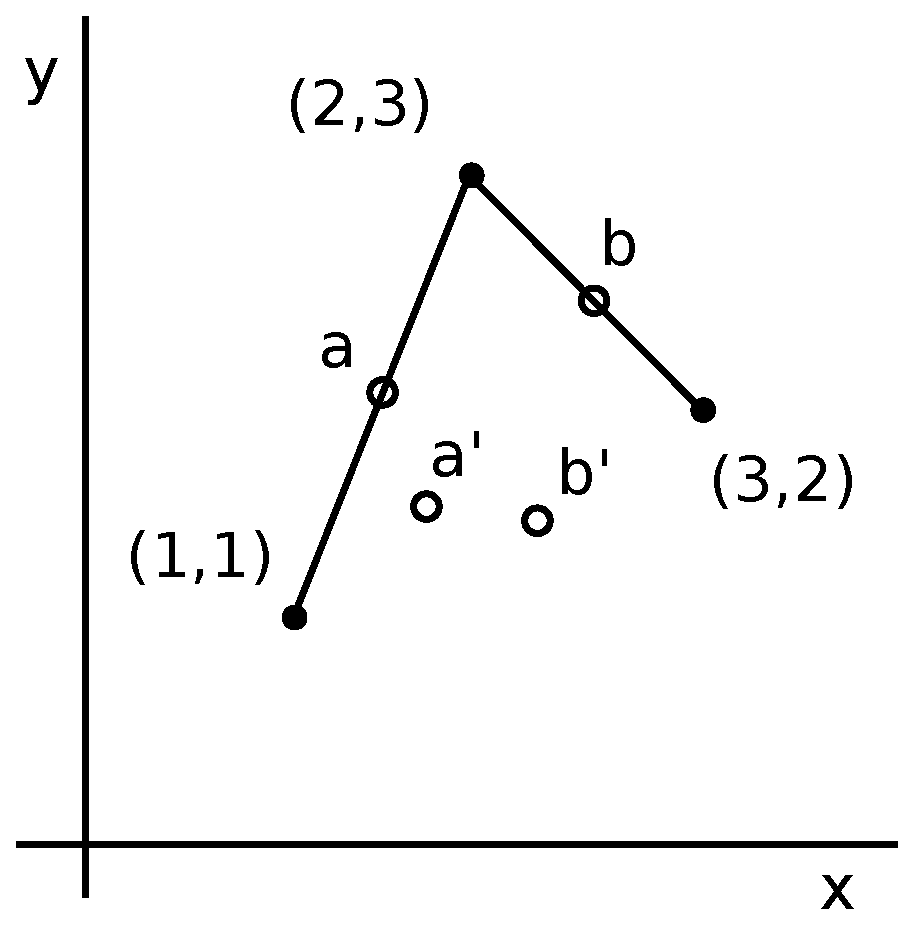
\includegraphics[width=\linewidth]{fig/interpolation-cartesian.eps}
    \caption{Cartesian Trajectory}
  \end{subfigure}
  \begin{subfigure}[H]{0.45\linewidth}
    \def\svgwidth{\linewidth}
    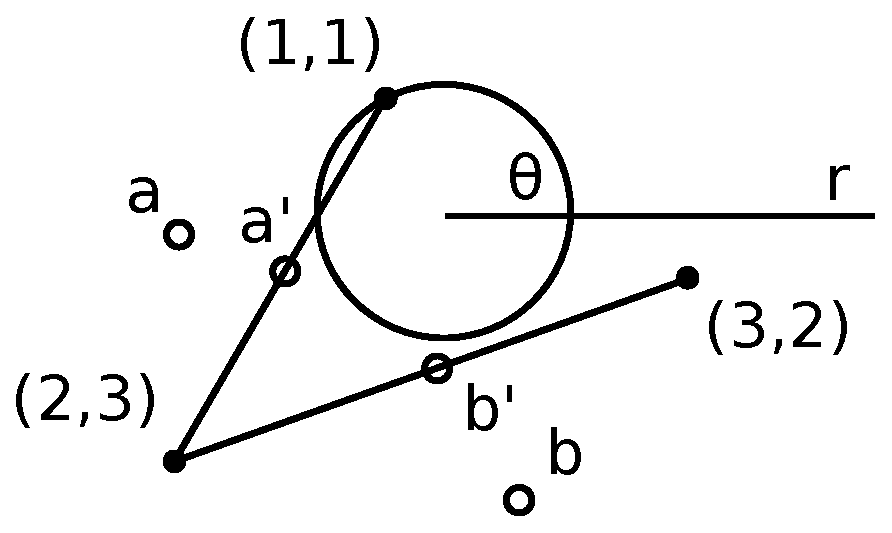
\includegraphics[width=\linewidth]{fig/interpolation-radial.eps}
    \caption{Radial Trajectory}
  \end{subfigure}
  \caption{Example of effect of spatial geometry on interpolation}
\end{figure}

For instance, suppose we have three 2D symbols of which we want to draw a trajectory through. Consider two different spaces for conceiving those points: Cartesian (x, y) and Radial (r, $\theta$). Suppose we take the DFT of three points, i.e. as a trajectory without interpolation, in each of the two spaces.  Since the values of each point are exactly the same for both spaces, when examining the transform, there would be no way to tell which space it came from.  If instead we draw lines through the points and interpolate before taking the transform, we see clearly that the interpolated points differ between the two spaces, and so the transform of each trajectory will also be different.  In this way, the information about the geometry of the space can have an effect on the abstraction of the trajectory in that space.

\subsection{Types}
Since our conceptual spaces are represented as Hilbert spaces, interpolating a trajectory through a sequence of concepts is equivalent to regressing through the points of the space and sampling from that regression.  As such, we can employ any number of regression techniques from the literature to determine an appropriate trajectory.

\subsubsection{Connect the Dots}
Though not really regression per say, the simplest method for interpolating between points would be to just draw a straight line between them and sample from that line.  This method has the benefit of being very simple, and may prove to be near-equivalent to other methods if the number of interpolated points is low enough.

The problem with this method is that it is not continuously differentiable and therefore quite "sharp".  This would manifest in the DFT by resulting in high amplitudes at higher frequencies.  It is difficult to say a priori if this is desirable, but it seems in general that we would prefer smoother functions through these points to avoid this effects.

\subsubsection{Gaussian Regression (Kriging)}
One method for creating a smooth curve through these points is Gaussian Regression.  By thinking of the sequence of points as a multivariate Gaussian distribution, we can think of a distribution of trajectories or functions, i.e. a process, through these points.  By finding the mean function of this process we can find the maximum a posteriori trajectory of the process, resulting in the highest likelihood function through a sequence of points.  This method automatically avoids problems of overfitting inherent in higher-order transformation linear regression methods, though has the problem being computationally expensive.

By utilizing the square exponential kernel for Gaussian regression, the resulting curve will not only by the MAP curve, but also infinitely differentiable, meaning that it is hella smooth.  This smoothness results in a reduction of large high frequency amplitudes that could potentially happen in simpler methods like Connect-the-dots.



\chapter{Methods}
\include{tex/methods/methods}
\section{Methodology}

\subsection{Parameterization}

\subsection{Data}

\subsection{Experiments}

\section{Results}
\label{section:results}

\subsection{Category Reduction}
\label{section:category-reduction}

\begin{table}
\centering
\begin{tabular}{@{}llll@{}}
  \toprule
  Layer $\alpha$ & Instances & Categories & \% Reduction \\
  \midrule
  0 & 2841 & 605 & 78.7 \\
  1 & 1738 & 601 & 65.4 \\
  2 & 824 & 438 & 46.8 \\
  3 & 356 & 319 & 10.3 \\
  \bottomrule
\end{tabular}
\caption{Category Reduction}
\label{table:category-reduction}
\end{table}

Looking at table \ref{table:category-reduction}, we see that at each layer, there is a reduction in the number of symbols represented at that abstraction level.  At level 0, we see the largest reduction from instances to categories of 78.7\%.  A large portion of this reduction is due to the categorization of 'silence' -- that is, inaudible white noise -- that, from moment to moment, has distinct values that are extremely close together in space.  This can be seen at the beginning of the clip in Figure \ref{figure:category-flow}.

As the level of abstraction increases, the number of instances in that layer decrease due to segmentation.  In addition, categorization still occurs at each level, though the degree at which instances are categorized together also decreases.  This is due most significantly to the 'silence' categories being hierarchically categorized together into fewer categories, though, as we will see in the following sections, other non-silence categories are being grouped together as well.

\subsection{Category Flow}
\label{section:category-flow}

\begin{figure}
  \centering
  \includegraphics[width=\linewidth]{fig/category-flow-90.pdf}
  \caption{Category Flow of layers 0-3 with a Spectrogram}
  \label{figure:category-flow}
\end{figure}

The Category Flow diagram (Figure \ref{figure:category-flow}) illustrates the hierarchical categorization process. At each level, the word and syllable annotations boundaries are overlaid on top of the categories to easily discern where a certain sound should approximately begin and end.  The spectrogram is also displayed for visual comparison of the annotations and the actual signal.  In the category flow, each category is represented for its duration in the clip for each abstraction level, where each category has a spot on the y-axis -- that is, a category corresponds to a horizontal line on the plot.  In order to illustrate how transitions in a subordinate layer are abstracted into categories in the superordinate layer, the categories are ordered according to their maximum pair frequency such that categories that often appear in sequence are next to each other vertically.

In the category flow, we see that lower levels are quite noisy, with nearly all categories persisting for a single moment.  As we move up in abstraction, the flow flattens out and solidifies, meaning that trajectories from the subordinate layers are being categorized together in the superordinate layer.  As the abstraction level increases, we see a tendency for transitions between categories to flatten out into a smaller number of categories, where at the higher levels, these transitions flatten out completely into just one category.  By solidifying, we mean that the dispersed, noisy transitions found in the lower layers are categorized together in the upper layers, resulting in a "denser" category flow.

This process begins a bit in layer 2, but occurs much more frequently in layer 3.  This is most easily seen in the silent portion, marked \textit{h\#}, at the beginning of the clip.  Since this syllable is not actually silent because it contains faint white noise, the lower layers categorize these different moments of white noise separately, resulting in the ramp in categories at level 0.  Moving up the abstraction layers, their trajectories are categorized together into just a handful of categories at level 3.  This is evidence that the spectral representations of trajectories are consistently being categorized together if the trajectories they are representing are similar.

We can also see a few sections at level 3 where the categories or trajectories nearly line up with the syllable annotation boundaries.  For instance, the 's' syllable in the word 'suit' has been categorized into one category at this level, and the trajectory for the 'ao' syllable in the word 'wash' is clearly demarcated at the annotated boundaries.  One would expect that at the next level of abstraction, these trajectories would then become categories.

When examining all the abtractions layers as a whole, one can see noisy category transitions at the bottom layers become more consistent at the upper layers.  Even more, we can see that similar trajectories in lower layers are categorized together in upper layers.  This is evident in the 'striping' seen in lower layers -- perhaps a frequency beating artifact of the recording -- becoming a single category in upper layers.  This is seen most readily in the 's' syllable of the word 'suit', which exhibits striping at the lower levels.  Since these transitions are very similar, their trajectories and therefore spectral representations should be similar. Indeed, we see that at the upper levels these similar transitions are all categorized together, indicating that the categorization of spectral representations of trajectories behaves as expected as outlined in the theory.

\subsection{Category Distribution}
\label{section:category-distribution}

\begin{figure}
  \centering
  \includegraphics[width=\linewidth]{fig/category-distribution.pdf}
  \caption{Category Distribution of layers 0-3 going from right to left}
  \label{figure:category-distribution}
\end{figure}

 Since, especially at the higher levels, visualizing these high-dimensional categories is nigh impossible, the category distributions plot (figure \ref{figure:category-distribution}) shows the distribution of categories for a given dimension by showing how far away a given category is from the origin (i.e. the norm of the centroid of a category) on the x-axis, and the radius of the category on the y-axis.  This means points to the right of the distribution represent categories that are in general more distant from other categories, and points toward the top will have a larger inclusion radius $\rho$ and volume.

Looking at all of the distributions, one can immediately see a positive correlation between the remoteness (i.e. distance from the origin) of a category and its volume.  At each abstraction level, we see most categories are close together with a small volume, and as they move away from the origin, there volume also increases.  This is to be expected since the adaptive categorization tends to reduce the volume of categories with many members, and there are more instances near the origin than away from it.  Therefore, looking at the space as a whole, we see that the category density is high near the origin, and more sparse as one moves out.

It is also important to note that the adaptive categorization method employed here is not overly constraining the radii of each dimension.  If it were, instead of the linear trend we see here, the trend would shoot up to initial radius $\rho_0$ of the dimension and flatten out in an inverted-L shape.  This top-flattening not only results in most categories having nearly the same volume, but would also result in a larger amount of non-categorizable regions in the space; both of these qualities are undesirable.  In fact, the maximum posterior radius for each level is well below the initial radius, indicating that it is not a limiting factor in the categorization.  This shows that the adaptive categorization fills the space quite well, though more analysis would need be done to determine the analytical extent of the spatial covering, left to future research.

\subsection{Category Similarity}
\label{section:category-similarity}

\begin{figure}
  \centering
  \includegraphics[width=\linewidth]{fig/category-similarity-90.pdf}
  \caption{Category Similarity of Abstraction Layer 3}
  \label{figure:category-similarity}
\end{figure}

Since it is difficult to discern in the category flow (figure \ref{figure:category-flow}) if there is consistent categorization of similar sounds across the whole clip, the category similarity matrix (figure \ref{figure:category-similarity}) for abstraction level $\alpha = 3$ can be used instead.  At each moment in the clip the current category is compared with the category of every other moment in the clip, finding their distance, and representing closer categories with lighter shades and distant categories with darker shades.  Therefore, we see that diagonal is white, since the category of a moment has zero distance to itself.  Both axes of the matrix are also annotated with the words and syllables, like in the category flow, so that the similarity between different words and syllables of the clip can be compared.

Looking for light areas off the diagonal, there are three main areas of interest.  The first is at the intersection of 'she' and 'greasy'.  Clearly, the syllables of these words sound similar, so it makes sense that this area is lightly shaded and white.  Another white area is at the intersection of the words 'had' and 'in'.  Though in most accents these syllables of these words sounds quite different, the particular New England accent of this speaker has these words sounding similar -- something near 'hed' and 'en'. The other off-diagonal white area to call out comes at the intersection at the end of the words 'dark' and 'suit'.  For this accent, the ends of both of these words are unpronounced and are replaced with a stop, meaning they also qualitatively sounds quite similar.

Since similar sounding syllables are either in the same category or very close categories, this is evidence that categories semantically representing human speech syllables are beginning to emerge at this level.  Note that this emergence is occurring without any knowledge of this domain being human speech data, meaning that the general IDyOT processes behave as expected without specifying domain-specific information in the model.


\chapter{Discussion}
\section{Discussion}
\label{section:discussion}

\subsection{Addressing Categorical Inconsistencies}
\label{section:addressing-categorical-inconsistencies}

Though the category similarity matrix confirms that some similar-sounding syllables are either categorized together or at least near each other in the space, there are also confusing portions.  For instance, the entire word 'water' is categorized into a few very similar categories.  At higher levels of abstraction than seen here, one might expect that whole words would compose a single category, but since at abstraction level 3 we seem to be still mostly categorizing syllables and diphtongs, we would not expect the entire word to be one category.

This over-categorization may be due to two issues.  The first may be that the categorization is too eager in this location, resulting in different points being grouped together that should not be.  Though a significant amount of tuning was performed to find good initial radii for each layer, it's possible that a lower radius at this level would result in a more intuitive categorization for this particular region.

On the other hand, it may instead be due to the segmentation scheme employed in this implementation.  Here, we segment the stream at either a rise in entropy \textit{or} a rise in information content, resulting in numerous, relatively short segments.  Though there are a large number of segments, any given segment will not contain much information, by nature of its short length.  For a less eager segmentation, we could segment at a rise in just one of the measures.  This would result in fewer but longer segments with more information per segment. Though there would be fewer resulting categories from this reduced scheme, each category would be richer in that it represents more information, and may result in categories that consistently represent full syllables at this level of abstraction.

\subsection{Meaningful Categorizations}
\label{section:meaningful-categorizations}

That being said, though not perfect, we do observe the emergence of a few consistent categories that represent syllables at abstraction layer 3.  Since we also clearly see that similar trajectories are being categorized together in higher layers, it is a tenuous confirmation that the abstraction process as set forth in the theory behaves as intended.  We can see that even at a relatively low abstraction level 3, the hierarchical spectral representations of the speech signal are coalescing into categories that could be said to represent human speech sounds.  One could imagine, given a few more levels of abstraction and significantly more training, that the higher-level abstraction categories would become consistent, meaningful representations of the human speech signals they are learned from.

\subsection{Unified Approach to Perceptual Representation}
\label{section:unified-approach-to-perceptual-representation}

What makes these results exciting is not just that we are beginning to see the emergence of syllables as discrete categories, but the general applicability of this method.  Not only might we expect to see more complex elements of human speech such as words, sentences, and even syntax start emerge as categories in higher levels of abstraction, but the processes of segmentation, categorization, and abstraction are agnostic about the domain of the data in operation. That is, instead of using human speech signals as the raw input, another audio domain such as music could be used, as in IDyOM \citep{pearce2005construction}.  In general, just about any time-varying signal could be used instead.  Since other modes of perception such as vision can be modeled as time-varying signals, if consistent categories can be found for these human speech signals, perhaps semantically rich categories could be found for these other domains as well.  Doing so would uncover related semantics from different areas of perception, resulting in a more holistic coginitive architecture that ties in the multitude of domains of human experience.


\chapter{Conclusion}
\include{tex/conclusion/conclusion}
\section{Contributions}
\label{section:contributions}

There are a number of significant contributions from this thesis that move toward a formal implementation of the Information Dynamics of Thinking theory, which up until now, and not counting other IDyOT-like systems \citep{forth2016entraining}, was almost entirely a theoretical proposition.  Specifically, a significant portion of Chapter 3: Theory \& Implementation is work contributed by the author, though of course with guidance from the promoter and advisor, Prof. Dr. Dr. Geraint Wiggins.  A short review of specific contributions is presented in the following paragraph.  

Tensor rank promotion (section \ref{section:tensor-rank-promotion}) and element-wise independence (section \ref{section:elementwise-independence}) of the tensors produced in the abstraction process, though falling directly from the theory, were identified by the author. Though content sparsity was known prior in the theory, the problem of signal sparsity (section \ref{section:signal-sparsity}), in conjunction with the necessity for equal-shaped tensors falling from Hilbert space isopmorphism (section \ref{section:hilbert-space-isomorphism}) led to the need for interpolation (section \ref{section:interpolation}) and its proposed solution in regression sampling (section \ref{section:regression-sampling}).  In addition, the adaptive categorization (section \ref{section:adaptive-categories}) technique expanded on the idea of an inclusion radius and made it adaptive to the constituents of the category.

Beyond these theoretical contributions, this is the first, albeit limited, realized implementation of IDyOT that utilizes all three main processes: abstraction, segmentation, and categorization. As seen in the results, this is the first empirical analysis that spectral representations of meaning in the context of IDyOT, at least in human speech, can produce identifiable representations in a hierarchical manner.  This highly novel and general approach to perceptual representation could have far-reaching consequences, but here was the first empirical result that the whole theory might be viable.

\section{Limitations}
\label{section:limitations}

\subsection{Exponential Size of Category Representation}
\label{section:exponentil-size-category-represention}

The primary limitation encountered was due to the problem of tensor rank promotion (see section \ref{section:tensor-rank-promotion}).  With the brain being massively parallel, its possible that this exponential growth in the size of representation and the resulting spectral transform, is not a problem for the human mind.  However, even with significant parallelization of the categorization process, and using the Fast Fourier transform \citep{cooley1965algorithm} to group the spectral representations, the memory requirements alone became beyond extraordinarily large.

To ameliorate this, we repeatedly reduced the resolution of interpolation to hinder this growth, as well as capping the highest abstraction level to 3.  Unfortunately, this may have resulted in categories that are less informative overall, and we were not able to investigate higher level of abstraction, which would potentially yield consistent, semantically rich categories.

\subsection{Categorization Schemes}
\label{section:categorization-schemes}

The other major limitation was due to varying schemes that were tested in order to implement the categorization process.  Though signficant effort was put into finding different methods to not only adapt to the expontial growth in representation, but also the nature of the raw signal input, this was found to be too difficult to do \textit{a priori}.  Therefore, the adaptive categorization scheme (see section \ref{section:adaptive-categories}) was devised with the initial radius hyperparameter to limit the amount of manual tuning necessary for reasonable categorization.  That being said, the initial radii still had to be manually tuned to fit each level of abstraction for this particular type of input signal.

In addition, as larger training sets were run on the system, there was a corresponding increase in the number of categories produced.  This has a marked effect on the speed at which a new instance is processed since all categories in a space must be checked for candidacy.  In the future, consolidation techniques \citep{wiggins2019learning} can be employed to limit this monotonically increasing number of categories in a given layer.

\section{Future Work}
\label{section:future-work}

\subsection{Inner Products and Spatial Geometry}
\label{section:inner-products-spatial-geometry}

One of the most interesting proposals of IDyOT theory is that, since the inner product determines the geometry of the space, we can impose different semantics on a space simply by employing a different inner product \citep{wiggins2018creativity}. In this implementation, the only inner product used corresponds to the Frobenius norm (see section \ref{section:frobenius-norm}), so future work is needed to examine how the categorization, interpolation, and abstraction processes implemented here will be effected by choosing inner products that correspond to different semantics of the space.  For instance, there is evidence that humans represent the pitch space as a spiral \citep{deutsch2013psychology} and represent the color space as a spindle \citep{sivik1994color}.  Inner products could be chosen for a semantic space so that its geometry conforms to these semantics.

\subsection{Spectral Projectors and Reification}
\label{section:spectral-projectors-reification}

One of the main problems of this formalism comes from the use of the Fourier transform operator as the method of producing a spectral respresentation in abstraction.  Since tensor rank promotion results in exponentially larger representations of a category, the processing and memory requirements for a given category become huge after only a few levels of abstraction.  If instead a different formalism is used for a spectral representation instead of the Fourier transform, but can avoid tensor rank promotion, then we retain the spectral time-invariance necessary for abstraction without the computational overhead. Specifically, if instead of using a spectral \textit{operator} like the Fourier Transform, a spectral \textit{projector} could be used.  This would mean that the spectral representation of a trajectory would remain in the same rank Hilbert space at each level of abstraction, thereby avoiding the problem of tensor rank promotion.

An exciting corollary of using a projector instead of operator is that since the abstraction of a trajectory would land in the same Hilbert space, but separate conceptual space, a reification process could be defined.  By mapping that spectral representation back onto its subordinate layer, one could examine an reified abstraction of a trajectory in the same space as that trajectory!

%By imperfect analogy, this would be akin to finding that the spectral representation of a full sentence is equivalent to a single word.  Not only would the geometric properties of this relation be interesting to study, the semantic relation between a trajectory and its reification would be enlightening.


\bibliographystyle{plain}
\bibliography{thesis}

\end{document}
